\documentclass[margin=1mm]{standalone}
\usepackage[utf8]{inputenc}
\usepackage{amsmath}
\usepackage{amsfonts}
\usepackage{amssymb}
\usepackage{tikz}
\usetikzlibrary{calc,arrows,positioning,shapes,shapes.gates.logic.US,trees, backgrounds}

\begin{document}
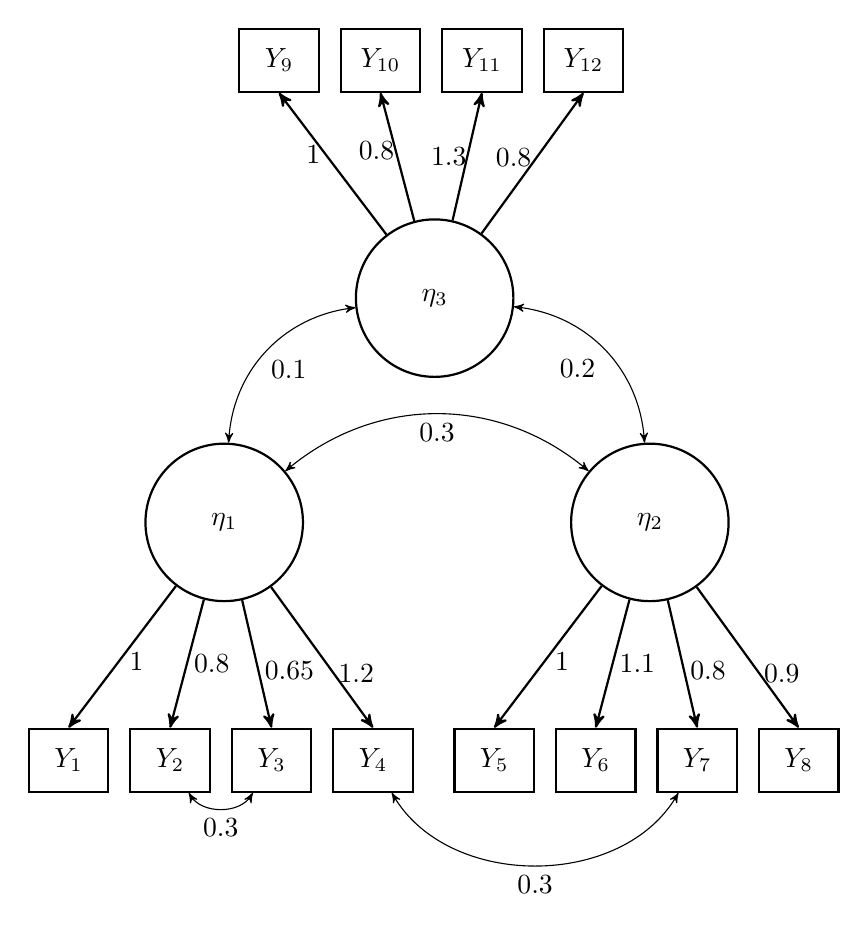
\begin{tikzpicture}[auto,scale=3,
	latent/.style={circle,draw,thick,text badly centered, inner sep=2pt,minimum size=20mm, text width=4.5em, fill=white},
	error/.style={circle,draw,text badly centered, inner sep=2pt,minimum size=10mm},
	manifest/.style={text centered, rectangle,draw,thick,inner sep=3pt,minimum height=8mm, minimum width=8mm, text width= 8 mm},
	manifestRot/.style={text centered, rectangle, draw, thick,inner sep=3pt, minimum width=7mm, text width= 7mm, minimum height=15},
	manifestfront/.style={rectangle,draw,thick,inner sep=0pt,minimum size=12mm, fill=white},
	ghost/.style={rectangle, inner sep=0pt,text centered,    minimum height=0mm, minimum width=5mm, text width= 5 mm},
	lcorr/.style={<->,>=stealth', bend right=40},
	rcorr/.style={<->,>=stealth', bend left=40},
	fcorr/.style={<->,>=stealth', bend left=40},
	ofcorr/.style={<->,>=stealth', bend right=60},
	ofcorr2/.style={<->,>=stealth', bend left=60},
	intercept/.style={regular polygon,
        regular polygon sides=3,draw,thick,inner sep=0pt,minimum size=10mm},
	mean/.style={regular polygon,regular polygon sides=3,draw,thick,inner sep=0pt,minimum size=10mm},
	paths/.style={->, thick, >=stealth'},
	variance/.style={<->, thick, >=stealth', bend left=270, looseness=2},
	varianceTop/.style={<->, thick, >=stealth', bend right=270, looseness=2},
	unique/.style={<->, thick, >=stealth', loop below=270, looseness=8},
	factvar/.style={<->, thick, >=stealth', loop right=270, looseness=8}
	] % End Creating Path Model Pieces
\tikzset{mystyle/.style={->,double=black}}


\node [manifest] at (0,0) (x1) {$Y_1$};
\node [manifest] (x2)  [right =.25cm of x1]   {$Y_2$};
\node [ghost]    (g1)  [right = 1.2cm of x1]  {};
\node [manifest] (x3)  [right =.25cm of x2]  {$Y_3$};
\node [manifest] (x4)  [right =.25cm of x3]  {$Y_4$};

\node [manifest] (x5)  [right =.50cm of x4]  {$Y_5$};
\node [manifest] (x6)  [right =.25cm of x5]  {$Y_6$};
\node [ghost]    (g2)  [right = 1.2cm of x5]  {};
\node [manifest] (x7)  [right =.25cm of x6]  {$Y_7$};
\node [manifest] (x8)  [right =.25cm of x7]  {$Y_8$};

\node [latent] (c1) [above = 2cm of g1]  {$\eta_1$};
\node [latent] (c2) [above = 2cm of g2]  {$\eta_2$};

%
\node [latent] (c3) [above right = 2cm of c1, xshift=-5]  {$\eta_3$};
\node [ghost]    (g3)  [above = 2cm of c3]  {};
\node [manifest] (x9)  [left =1.2cm of g3]  {$Y_9$};
\node [manifest] (x10) [right =.25cm of x9]  {$Y_{10}$};
\node [manifest] (x11) [right =.25cm of x10] {$Y_{11}$};
\node [manifest] (x12) [right =.25cm of x11] {$Y_{12}$};

\draw [paths] (c1) to node[pos=0.4, xshift=-5]  {$1$}   (x1.north);
\draw [paths] (c1) to node[pos=0.35, xshift=-3]  {$0.8$}   (x2.north);
\draw [paths] (c1) to node[pos=0.7, xshift=-3]  {$0.65$}   (x3.north);
\draw [paths] (c1) to node[pos=0.75, xshift=-7]  {$1.2$}   (x4.north);

\draw [paths] (c2) to node[pos=0.4, xshift=-5]  {$1$}   (x5.north);
\draw [paths] (c2) to node[pos=0.35, xshift=-3]  {$1.1$}   (x6.north);
\draw [paths] (c2) to node[pos=0.7, xshift=-3]  {$0.8$}   (x7.north);
\draw [paths] (c2) to node[pos=0.75, xshift=-7]  {$0.9$}   (x8.north);

\draw [paths] (c3) to node[pos=0.7, xshift=7]  {$1$}   (x9.south);
\draw [paths] (c3) to node[pos=0.7, xshift=5]  {$0.8$}   (x10.south);
\draw [paths] (c3) to node[pos=0.35, xshift=5]  {$1.3$}   (x11.south);
\draw [paths] (c3) to node[pos=0.4, xshift=7]  {$0.8$}   (x12.south);

\draw [fcorr] (c1) to node[below]{$0.3$} (c2);
\draw [fcorr] (c1) to node[below, xshift=8]{$0.1$} (c3);
\draw [lcorr] (c2) to node {$0.2$} (c3);


% error covariances
\draw[ofcorr] (x2) to node[below] {$0.3$} (x3);
\draw[ofcorr] (x4) to node[below] {$0.3$} (x7);
\end{tikzpicture}
\end{document}